\chapter{Background}
\label{chap:background}


	% >>> META INFO START:

	\besk{ Surveying of past and related work }

	\besk{ Clustering and classifications of main concepts and ideas used in the thesis } \nl

	% <<< META INFO STOP.


\section{Taking inspiration from psychology}


	% >>> META INFO START:

	\gjor{ Hent inn Essay-materiale inn hit }

	\gjor{ Merge 1) Essay . Conceptual Framework med 2) ``\tcol{self awareness scope (i.e. individual robots are aware of and susceptible to a larger number of neighbouring robots and their transmitted ``fire'' signals)}'' } \nl

	% <<< META INFO STOP.


% <<< \section END.



\section{Taking inspiration from natural phenomena}
The intriguing, diverse, and complex phenomena of nature have for long served as exciting inspirations to human engineers and researchers [ant-colonies, boids, swarms, beeclust]. From taking inspiration when designing a robot traversing one of the most challenging terrains to traverse through, granular surfaces like sand that is, from e.g. zebra-tailed lizards able to run up to 5 meters per second (normally in desert sand) \cite{sandbots}, to ... Such phenomena have been subject to considerable study and modelling—and have in fact created entire scientific fields \cite{biomimetics, bionics} in which principles from various science- \& engineering-diciplines are applied to the physical systems and machines having functions that mimic biological processes, as well as biological processes serving as great sources of inspiration for the engineered systems; \textit{Biomimetics} and \textit{Bionics}, that is. One branch of these types of natural phenomena observed and studied is the biological pulse-coupled oscillators \cite{russerMinimalAssumptionsReferanser}. An example of such biological pulse-coupled oscillators found in nature is the synchronously flashing fireflies, as e.g. can be seen in a dark forest in Figure \ref{fig:synched_fireflies_phenomenon}.

\begin{figure}[!ht]
	\centering
	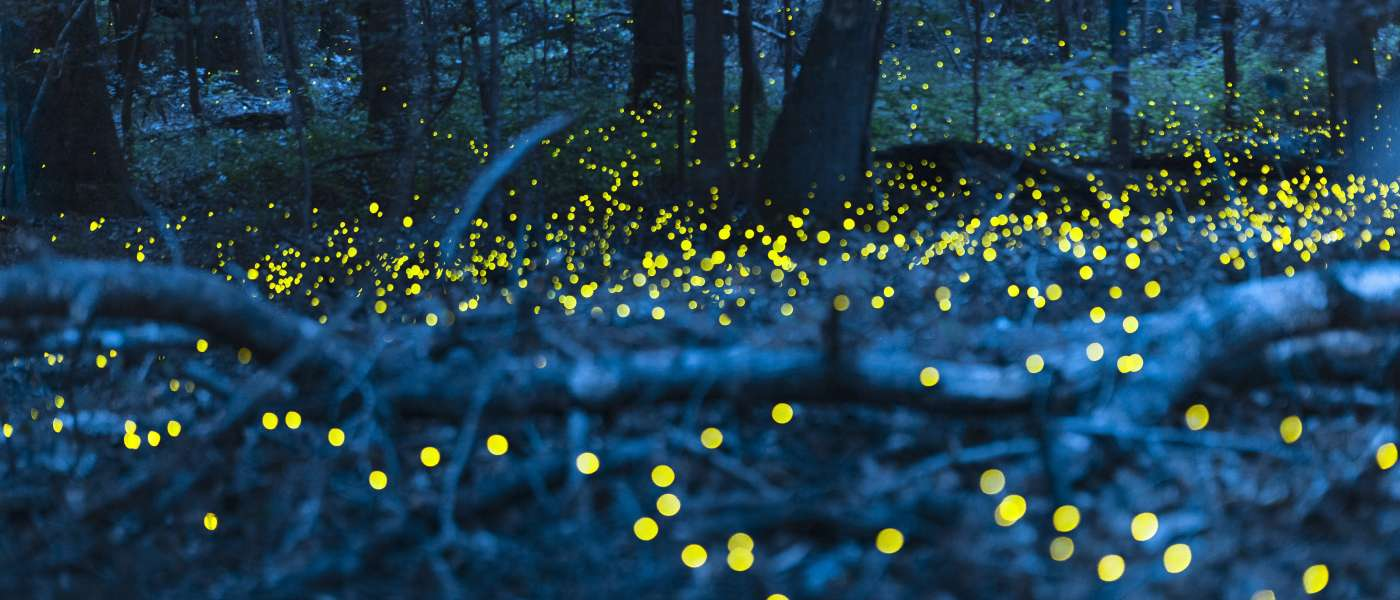
\includegraphics[width=0.9\linewidth]{Assets/DocSegments/Chapters/Background/Figures/Photos/synchronized_fireflies_phenomenon.jpg}
	\caption[Picture of fireflies flashing synchronously in a US National Park]{Synchronous fireflies at Congaree National Park, United States. Photo: @columbiasc + @\_flashnick (fotnote).} % ELLER F.EKS. {Copyright ©Blabla Corporation, David Thorvaldsen}
	\label{fig:synched_fireflies_phenomenon}
\end{figure}

This phenomenon has inspired scientists like Mirollo \& Strogatz \cite{mirollo_strogatz_PCO_synch} and in later time Kristian Nymoen et al. \cite{nymoen_synch}, to model and replicate this natural phenomenon in human-engineered systems. Given the periodic and repeating nature of the flashing/firing of the fireflies, modelling a firefly has been done by looking at each firefly as a periodic signal or oscillator. This work \cite{mirollo_strogatz_PCO_synch, nymoen_synch} then ties into the broader work on synchronizing oscillators which has been subject to study for some time now []. What separates Mirollo-Strogatz and K. Nymoen's approaches from these other and previous oscillator-synchronizing methods, is mainly that here the oscillators are \textit{pulse-coupled} (which the fireflies also can be said to be), as opposed to the more ``standard'' and constraining \textit{phase-coupled} oscillators. Additionally, K. Nymoen's approach accounts for synchronizing initially heterogenous frequencies as well.

% <<< \section END.



\section{Signals and their responses}


	% >>> META INFO START:

	\gjor{Forklare hva et signal eller et (lyd-)signal/waveform egentlig er (ift. harmonics/harmonic wave/overtones (og deres typiske integer-relationship frekvenser), og hvis tid timbre med varierende frekvenser (jf. Jay Eller hva han Andriy Burkov eller hva han het anbefalte), amplitude/gain, envelope/attack-decay)}

	% <<< META INFO STOP.


Signals, in various forms, are omnipresent in our world, whether we notice it or not. They are used for guidance: e.g. traffic-lights send visual light-signals to drivers to ensure traffic-flow and collision-avoidance; sirens and alarms fire away with the loudest of audio-signals (sounds) so that its listeners will get out of harms way; our nerves send pain-signals through our nervous-system if we touch something burning hot to ensure we do not damage our hand severely. If you have ever tried to make a scary sound to scare away an animal—like a cat or crow—they might in fact flee from you if they think your audible signal was scary enough for them.

A signal can also be called a waveform.

	\subsection{Amplitude}
	\begin{figure}[h!]
		\centering
		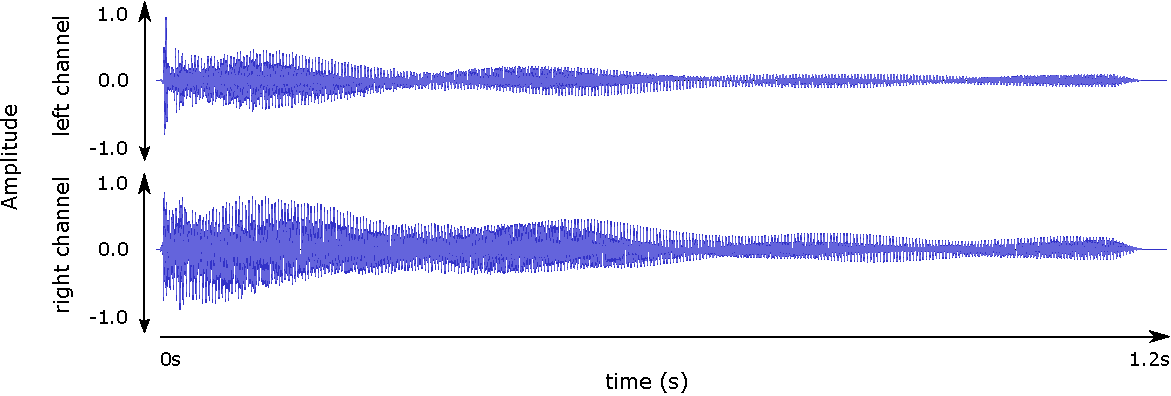
\includegraphics[width=\linewidth]{Assets/DocSegments/Chapters/Background/Figures/Illustrations/waveform.pdf}
		\caption[An audible waveform explained.]{An audible stereo- (hence the two channels, one for each ear) waveform, being a digitally created harp-sound (as further described in \ref{subsec:fire_signal}). The more positive or negative the amplitude is, the louder the audio-signal is.}
		\label{fig:waveform}
	\end{figure}


	\subsection{Frequency}
		\subsubsection{Spectra / Spectrograms}

% <<< \section END.



\section{Oscillators and oscillator-synchronization}


	% >>> META INFO START:

	\gjor{ Beskriv dette så godt at du kan snakke fritt om oscillatorers \textbf{faser} og \textbf{frekvenser} senere (i Implementation f.eks.), spesielt i tilfelle for noen ikke har vært borti det før, eller tatt et Signalbehandlings-kurs }

	\gjor{ Skill på Pulse-coupled Oscillators, og Phase-coupled Oscillators. Nevn fordelene, spesielt for roboter, med å synkronisere seg basert på diskret tid [Sandsbots-paperet Kyrre sendte deg (iaff. slutt-tabellen), SandBots-arkitekturen som åpner for lave oppdaterings-rater], sammenliknet med kontinuerlig tid }

	\besk{ Teori og nyere cutting-edge/state-of-the-art metoder for fase-/frekvens-synkronisering i oscillatorer og liknende. Se Kristian Nymoens referanser \cite{nymoen_synch} og artikler funnet i denne veinen } \nl

	% <<< META INFO STOP.


Oscillators have been used to implement and model a plethora of systems, also biological ones, ranging from designing the locomotion-patterns of swimming robot-amphibia through central pattern generators \cite{ijspeert_cpg}, ..., and as we have already established, modelling synchronously flashing or firing fireflies.
	
	
	\subsection{Phase and frequency}
	Much of the terminology from \cite{nymoen_synch} is used here. An oscillator $i$ is characterized by its \textit{phase} $\phi_i(t)$, which is—at the start of its periodic signal period—initialized to 0 and evolves towards 1 at a rate which is called the \textit{frequency} of the oscillator. So, in mathematical terms, the frequency $\omega_i(t)$ is then given by:
	
	\begin{equation}
	\label{phase_freq}
		\omega_i(t) = \frac{d \phi_i(t)}{d t} .
	\end{equation}

	When oscillator $i$'s phase is equal to 1 (i.e. when $\phi_i(t)=1$, or when the periodic signal period is over), we say oscillator $i$ has \textit{phase-climaxed}.
	
	An oscillator-period $T$ is defined as the inverse of the oscillator-frequency $\omega$. In mathematical terms:
	
	\begin{equation}
	\label{period_freq}
		T = 1/\omega .
	\end{equation}
	
	
	\subsection{Phase-adjustment}
	
	% >> META INFO START:
	
		\gjor{ Muligens inkluder introen i Section \ref{sec:phase_methods} her også (eller bare her?) }
		
		\besk{\tcol[gray]{(Hvis relevante og ønskede)} Tidligere metoder til Fase-synkronisering i oscillatorer (puls- og/eller fase-koplede)}
	
	% << META INFO STOP.
	
		\subsubsection{Mirollo-Strogatz's ``standard'' phase adjustment} % or phase synchronization, or phase updates
		\label{mirollo_strogatz_phase_adjust}
		
		One approach having been used to achieve this in the past is Mirollo-Strogatz's ``Standard'' phase-adjustment in oscillators \cite{mirollo_strogatz_PCO_synch}.
		
		Each musical agent gets a new phase, $\phi(t^+) = P(\phi(t))$, accoring to the \textbf{phase update function \eqref{strog_phase}} upon perceiving a ``fire''-event from one of the other musical nodes:
		
		\begin{equation}
		\label{strog_phase}
			\phi(t^+) = P(\phi(t)) = (1 + \alpha)\phi(t)	,
		\end{equation}
		
		where $\alpha$ is the pulse coupling constant, denoting the strength between nodes \cite{nymoen_synch}, $t^+$ denotes the time-step immediately after a ``fire''-event is heard, and $\phi(t)$ is the old frequency of the agent at time $t$. So, if e.g. $\alpha = 0.1$, then a musical agent's new and updated phase, immediately after hearing a ``fire''-signal from another agent, will be equal to $\phi(t^+) = P(\phi(t)) = (1 + 0.1)\phi(t) = 1.1\phi(t)$. 110\% of its old phase $\phi(t)$, that is. Hence, and in this way, the agent would be ``pushed'' to fire sooner than it would otherwise (as nodes fire once they have reached phase-climax $\phi(t)=1$).
	
	
	\subsection{Frequency-adjustment}
	
	% >> META INFO START:
	
		\gjor{ Muligens inkluder introen i Section \ref{sec:frequency_methods} her også (eller bare her?) }
		
		\besk{ \tcol[gray]{(If relevant and wanted)} Previous approaches to Frequency-synchronization in oscillators (pulse- and/or phase-coupled) [nymoen-referanser e.g.] where the oscillators's frequencies are either equal and fixed, or where frequencies are bound to initialize and stay within a fixed interval/range. }
		
		\besk{ \tcol[gray]{(If it exists)} A ``simpler'' frequency synchronization approach, to solve the phase and frequency ($\phi$ \& $\omega$) problem with, without any self awareness components }
	
	% << META INFO STOP.
	
% <<< \section END.
	
	

\section{Musical robots in music technology systems}


	% >>> META INFO START:

	\gjor{ Hent inn Essay-materiale om music technology systems her, spesielt om Solojam og kanskje Nymoen et al.s Firefly-system kjapt også (for å få en første idé før du går mer i detalj på dette systemet i \textbf{Baseline}) }

	% <<< META INFO STOP.


M. J. Krzyzaniak and RITMO's musical robots, the Dr. Squiggles, have been used in various music technology systems previously (fotnote) \cite{dr_squiggles}. Corresponding 3D-models of these robots were designed by Pierre Potel \cite{pierre_potel} and are reused, with permission, for the simulation system designed during this thesis project.

% <<< \section END.